This section explains the results of the project in \ref{subsec:results} and evaluate on the results in \ref{subsec:evaluation}.

\subsection{Results}
\label{subsec:results}
This section contains results for both the preprocessing and the two classification algorithms and their performance.

\subsubsection{Preprocessing}
The preprocessing was done in the following steps.
Initially the images was downscaled to 100 pixels width.
Images was normalized using Z-Score normalization resulting in the right image of Figure \ref{fig:step1}. By normalizing the images the contrasts becomes greater and this will ease the separation.
In the next step, the image is smoothed with a Gaussian smoothing algorithm with a sigma level of 2. This equalizes the values of the individual pixels a bit and thereby make neighboring pixel more alike.
When these steps are done, two features are extracted from each pixel.
These features are the redness and a gray scale value.
The features are then used for the K-Means clustering algorithm.
The clusters are constructed using Euclidean distances. Further is the algorithm constructed to build 4 different clusters.
The reason for using four clusters, is that it is expected that water, water splashes, whale and 'garbage' will be in their own separate cluster.

When the clusters are created the next step is to identify which cluster(s) the whale have been added to.
This is done by finding the cluster which has the highest rate of redness within it. This works for most of the images but not all. In some images the contrast between whale and water is not high enough or the light when the image was taken makes the water splashes red. When this happens, the correct cluster is chosen by calculating the center of gravity in the image. After the center of gravity is calculated the cluster in which it is placed is picked, if the size of that cluster is between 5 \% and 20 \% of the total. This picks the correct cluster with an accuracy of around 50 \%.
When it fail to find a cluster, a cluster matching the size for 10-15 \% of the total image is taken \footnote{Note that the last approach might choose a wrong cluster, and cannot be validated, which is why the two other approaches are preferred}. 

When one or more cluster is chosen, everything not in that cluster is filtered out from the original smoothed image as seen in Figure \ref{fig:step3} right. The whole process is then repeated once more in order to filter out some few water pixels which was gathered in the whale cluster.
After the second round a minimum bounding box is calculated around the whale cluster, and the image is then cropped.

\begin{figure}
\centering
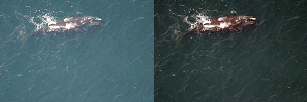
\includegraphics{Images/preprocess1}
\end{figure}

\subsubsection{Random Forest}
The Results for Random Forest is split into two sections. As there has been conducted classification for both data which was just resized and data which has been additionally preprocessed before resizing.

\paragraph{The Resized Data}
\label{par:rf-resized}
Shown in Figure \ref{fig:random-forest-resized}, an averaged result of 3 fold cross validation. The graph is shown with a one-tailed 95\% confident interval with a degree of freedom on 3. The criteria of interest is the potential worst performance of the model. Which is the upper line of the embedded error bar on the graph at each point. The cutoff line defines the performance at random selection, which is 1 / 447. 

Each validation point for the chart correspond to the number of trees in the forest, plus 1 additional tree. So for validation point ``5'', the model has 6 trees.

The performance of the test set for Figure \ref{fig:random-forest-resized} do for each validation point have a \emph{significant better performance} than choosing random selection, see Table \ref{tab:result-conclusion}.

The training set does significant better than the test set, but just states that the model is overfitted and should be trained against more observations to introduce more variety.

\begin{figure*}
  \centering
    \begin{subfigure}{.5\linewidth}
      \centering
      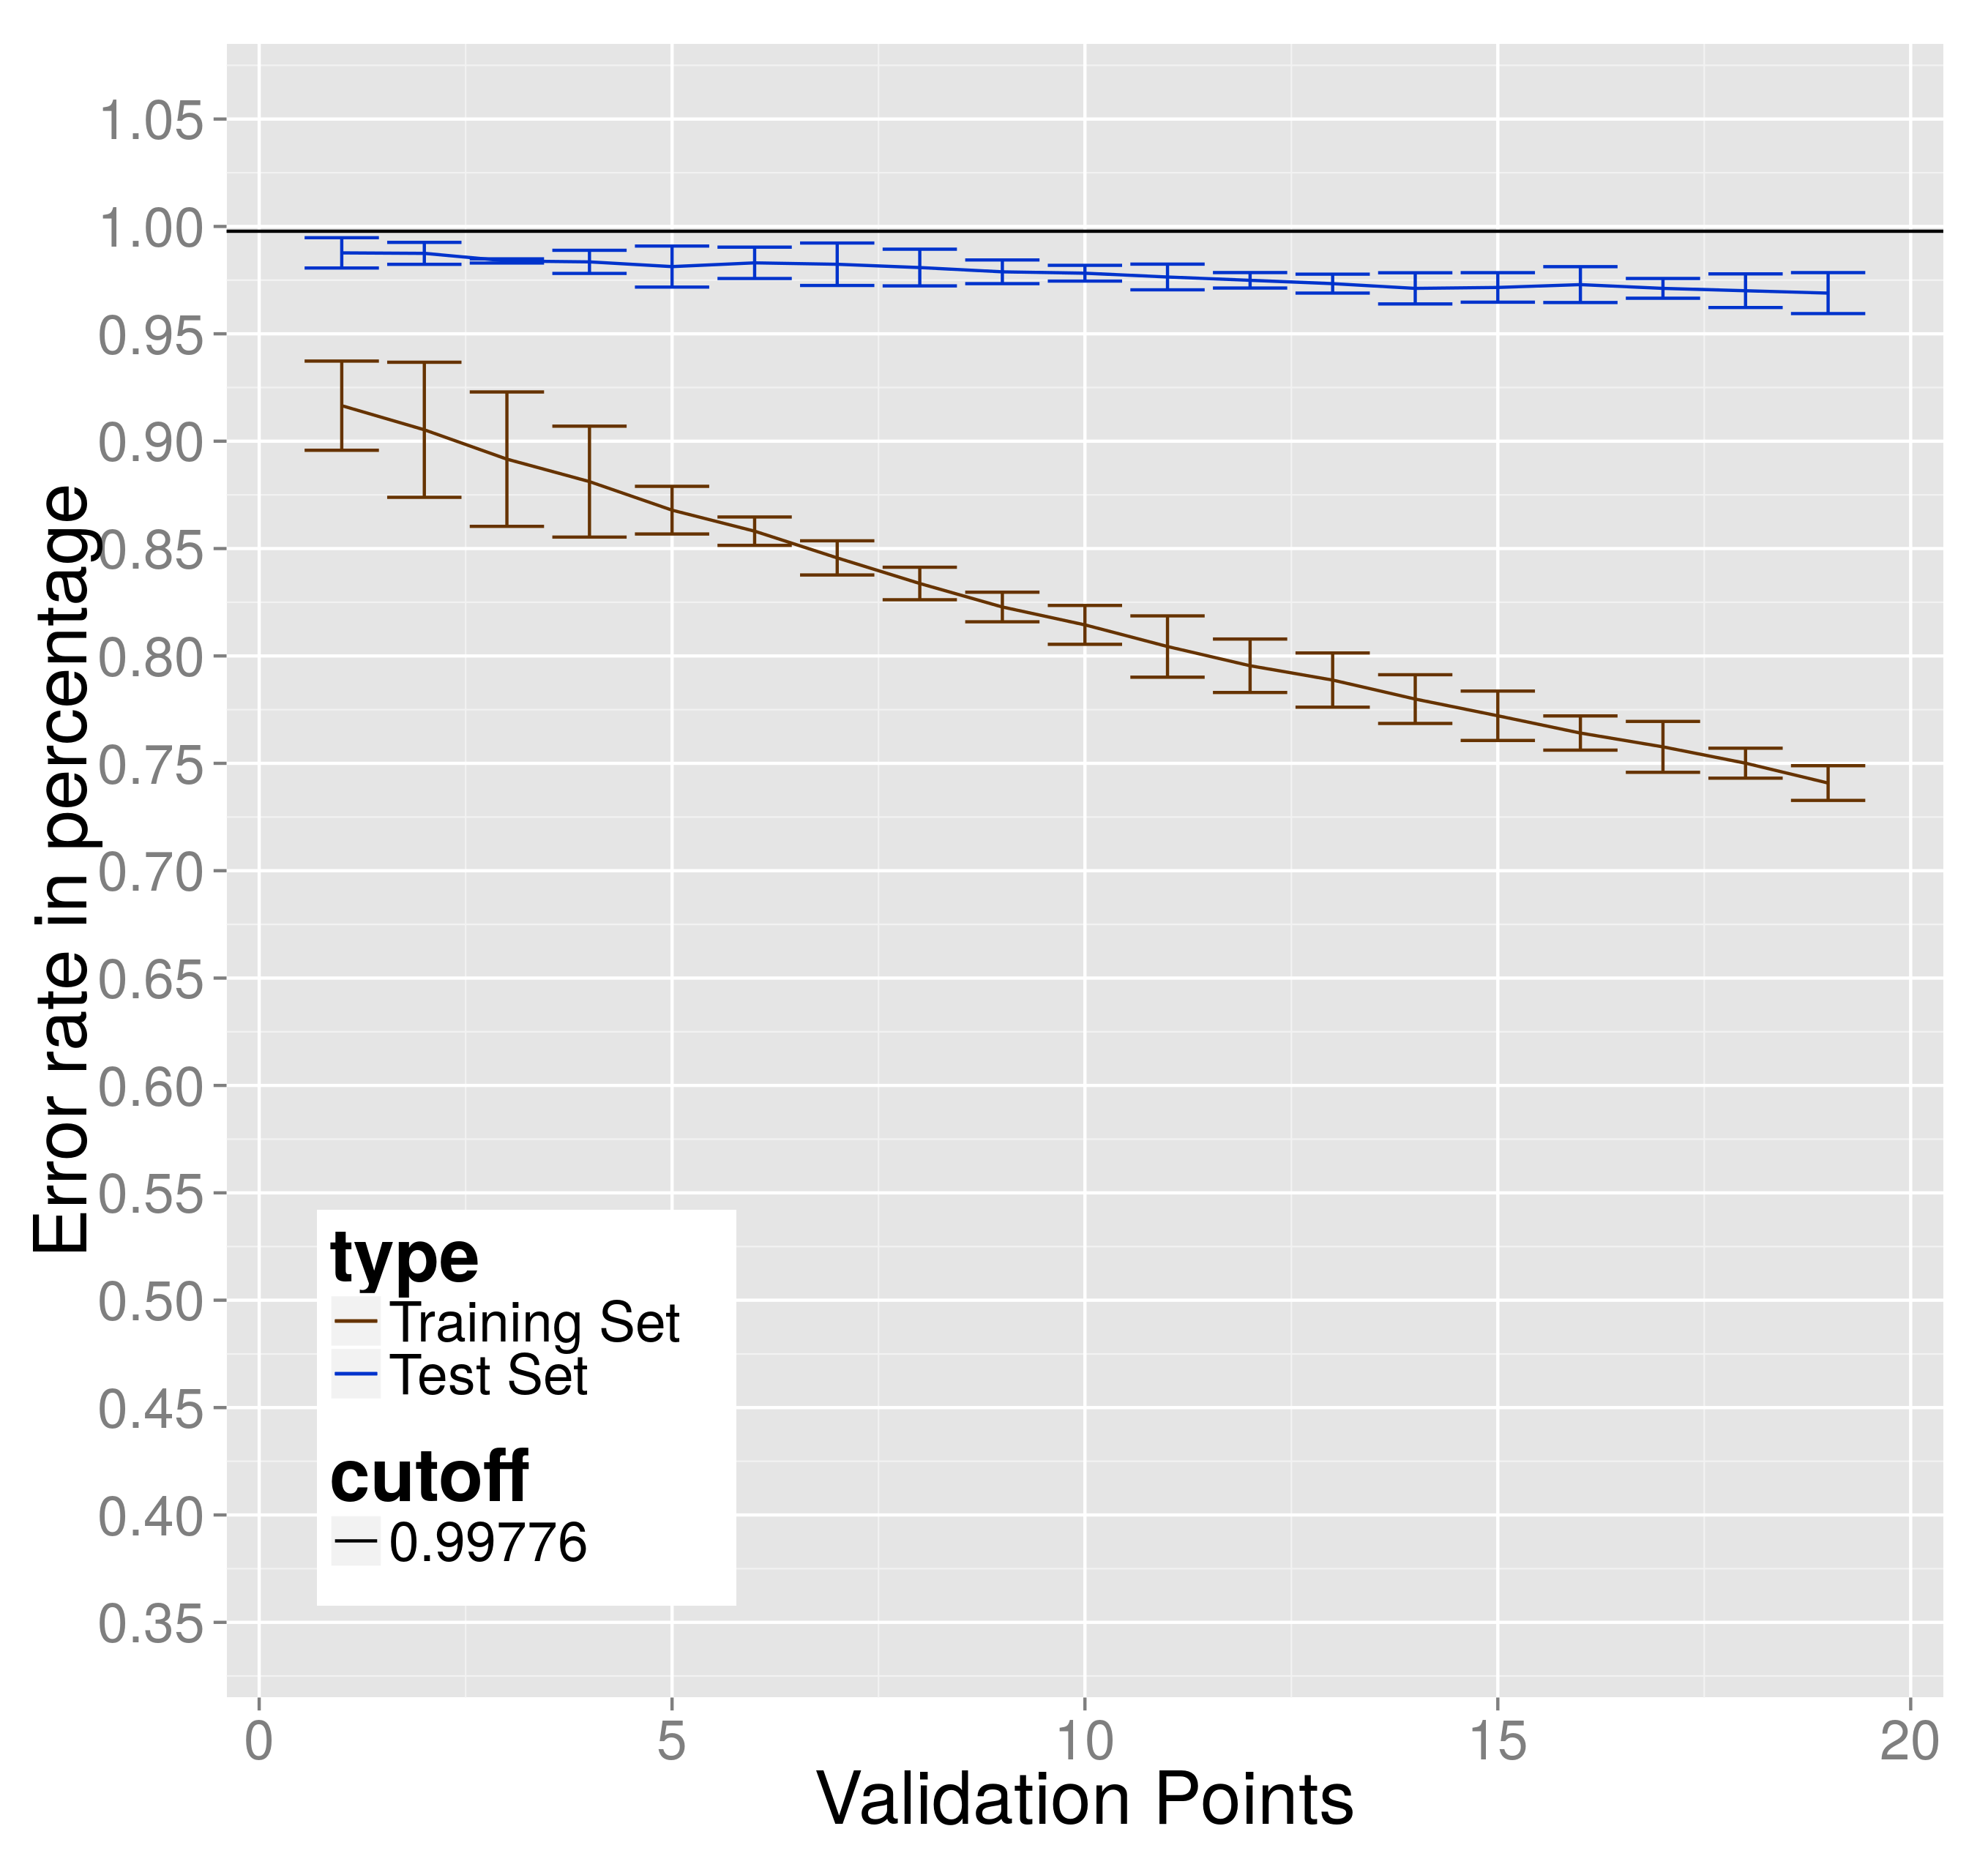
\includegraphics[width=0.95\linewidth]{Images/DRFraw}
      \caption{Without preprocessing}
      \label{fig:random-forest-resized}
    \end{subfigure}%
    \begin{subfigure}{.5\linewidth}
      \centering
      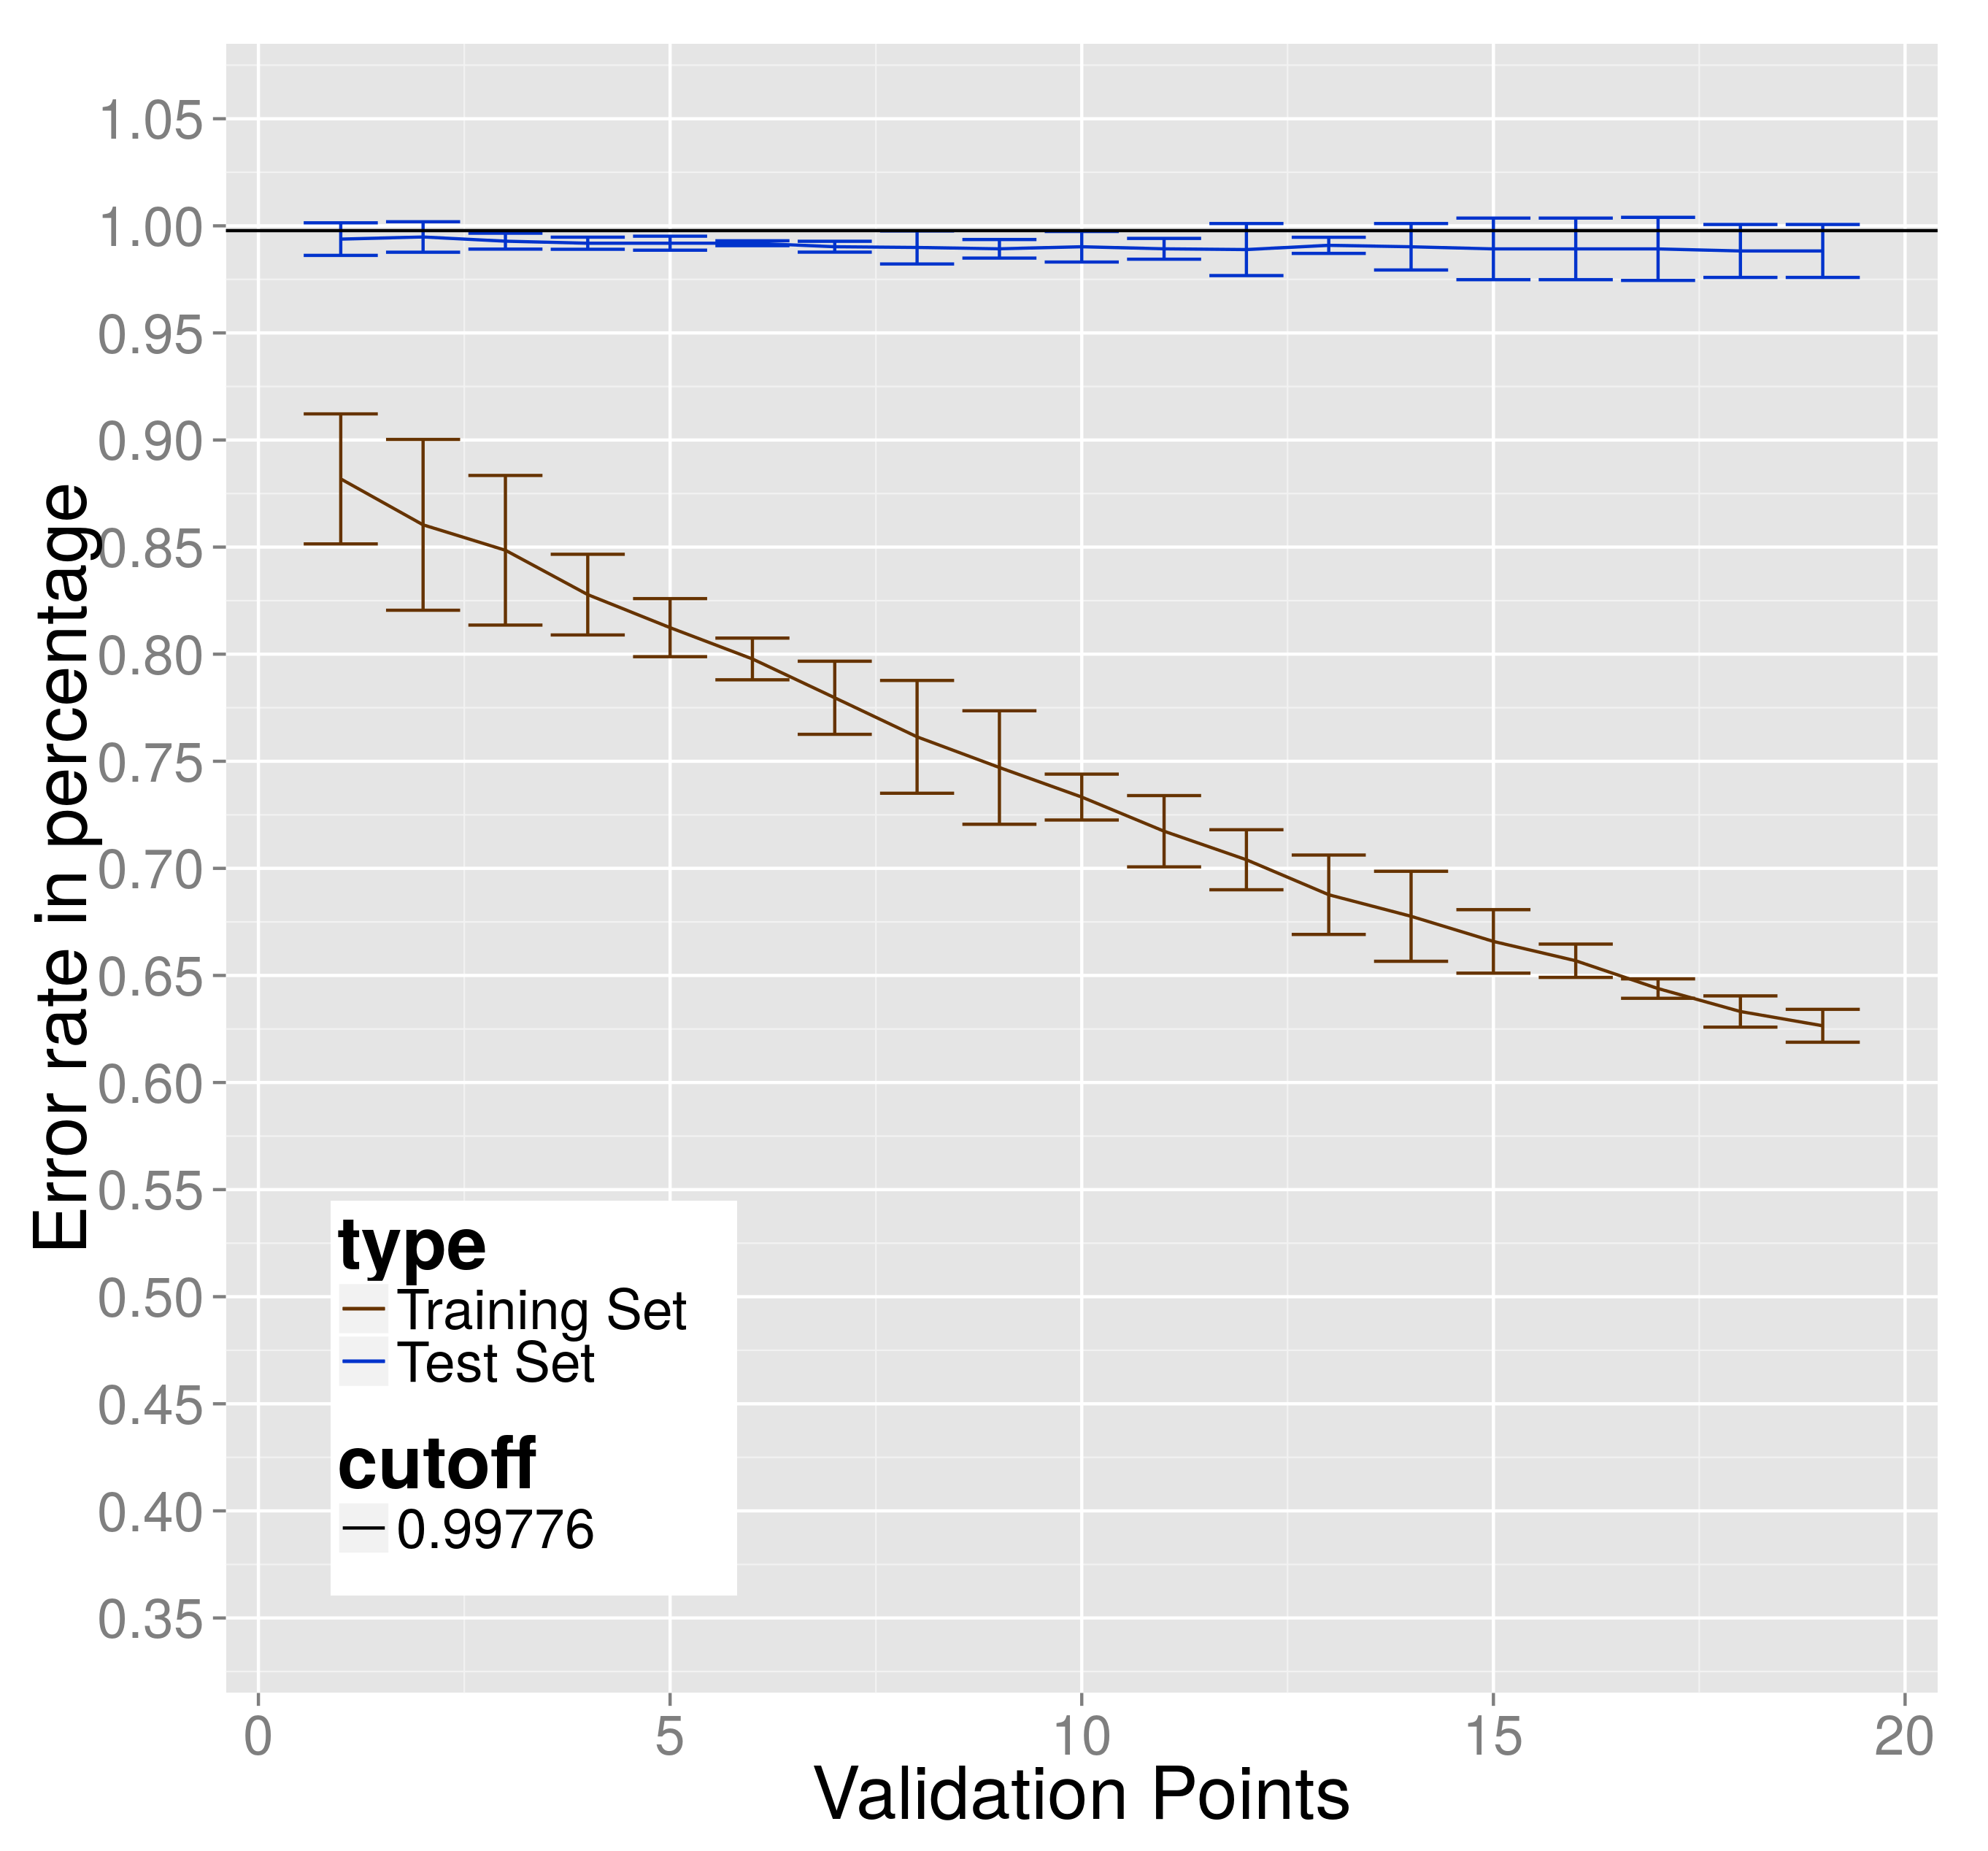
\includegraphics[width=0.95\linewidth]{Images/DRFpreprocessed}
      \caption{With preprocessing}
      \label{fig:random-forest-preprocessed}
    \end{subfigure}
  \caption{The results for Random Forest}
  \label{fig:random-forest}
\end{figure*}

\paragraph{The Preprocessed Data}
Shown in Figure \ref{fig:random-forest-preprocessed} follow the same conditions with 3 fold cross validation, one-tailed 95\% confident interval with degree of freedom on 3, as seen at \ref{par:rf-resized}.

The only different is the data input which uses the preprocessed data instead.
The test set \emph{do not} have a significant better performance than random selection, but do have some sweet spots at some amount of trees which seems better, but might as well be due to the limited amount of folds, see Table \ref{tab:result-conclusion}.

The training set shows the same issues as the only resized images shown in Figure \ref{fig:random-forest-resized}, also explained in \ref{par:rf-resized}.

\subsubsection{Neural Network}
\label{subsubsec:neuralnetwork}
This section contains the results from the neural network model using both the resized and the preprocessed datasets.

\paragraph{The Resized Data}
in Figure \ref{fig:nn-resized} shows two non-static lines and a static cutoff line.
The static cutoff line represent random selection for a correct classification, where as the two other lines show the test and training sets performance against the model at given validation points. Additionally a one-tailed 95\% confident interval at 3 degrees of freedom is shown as the error bar at each validation point for both lines.

The test set \emph{do not} have a significant better performance than random selection
, see Table \ref{tab:result-conclusion}.

The training set do have a \emph{significant better performance} against the model compared to the test set, which shows overfitting also mentioned in \ref{par:rf-resized}


\begin{figure*}
  \centering
    \begin{subfigure}{.5\linewidth}
      \centering
      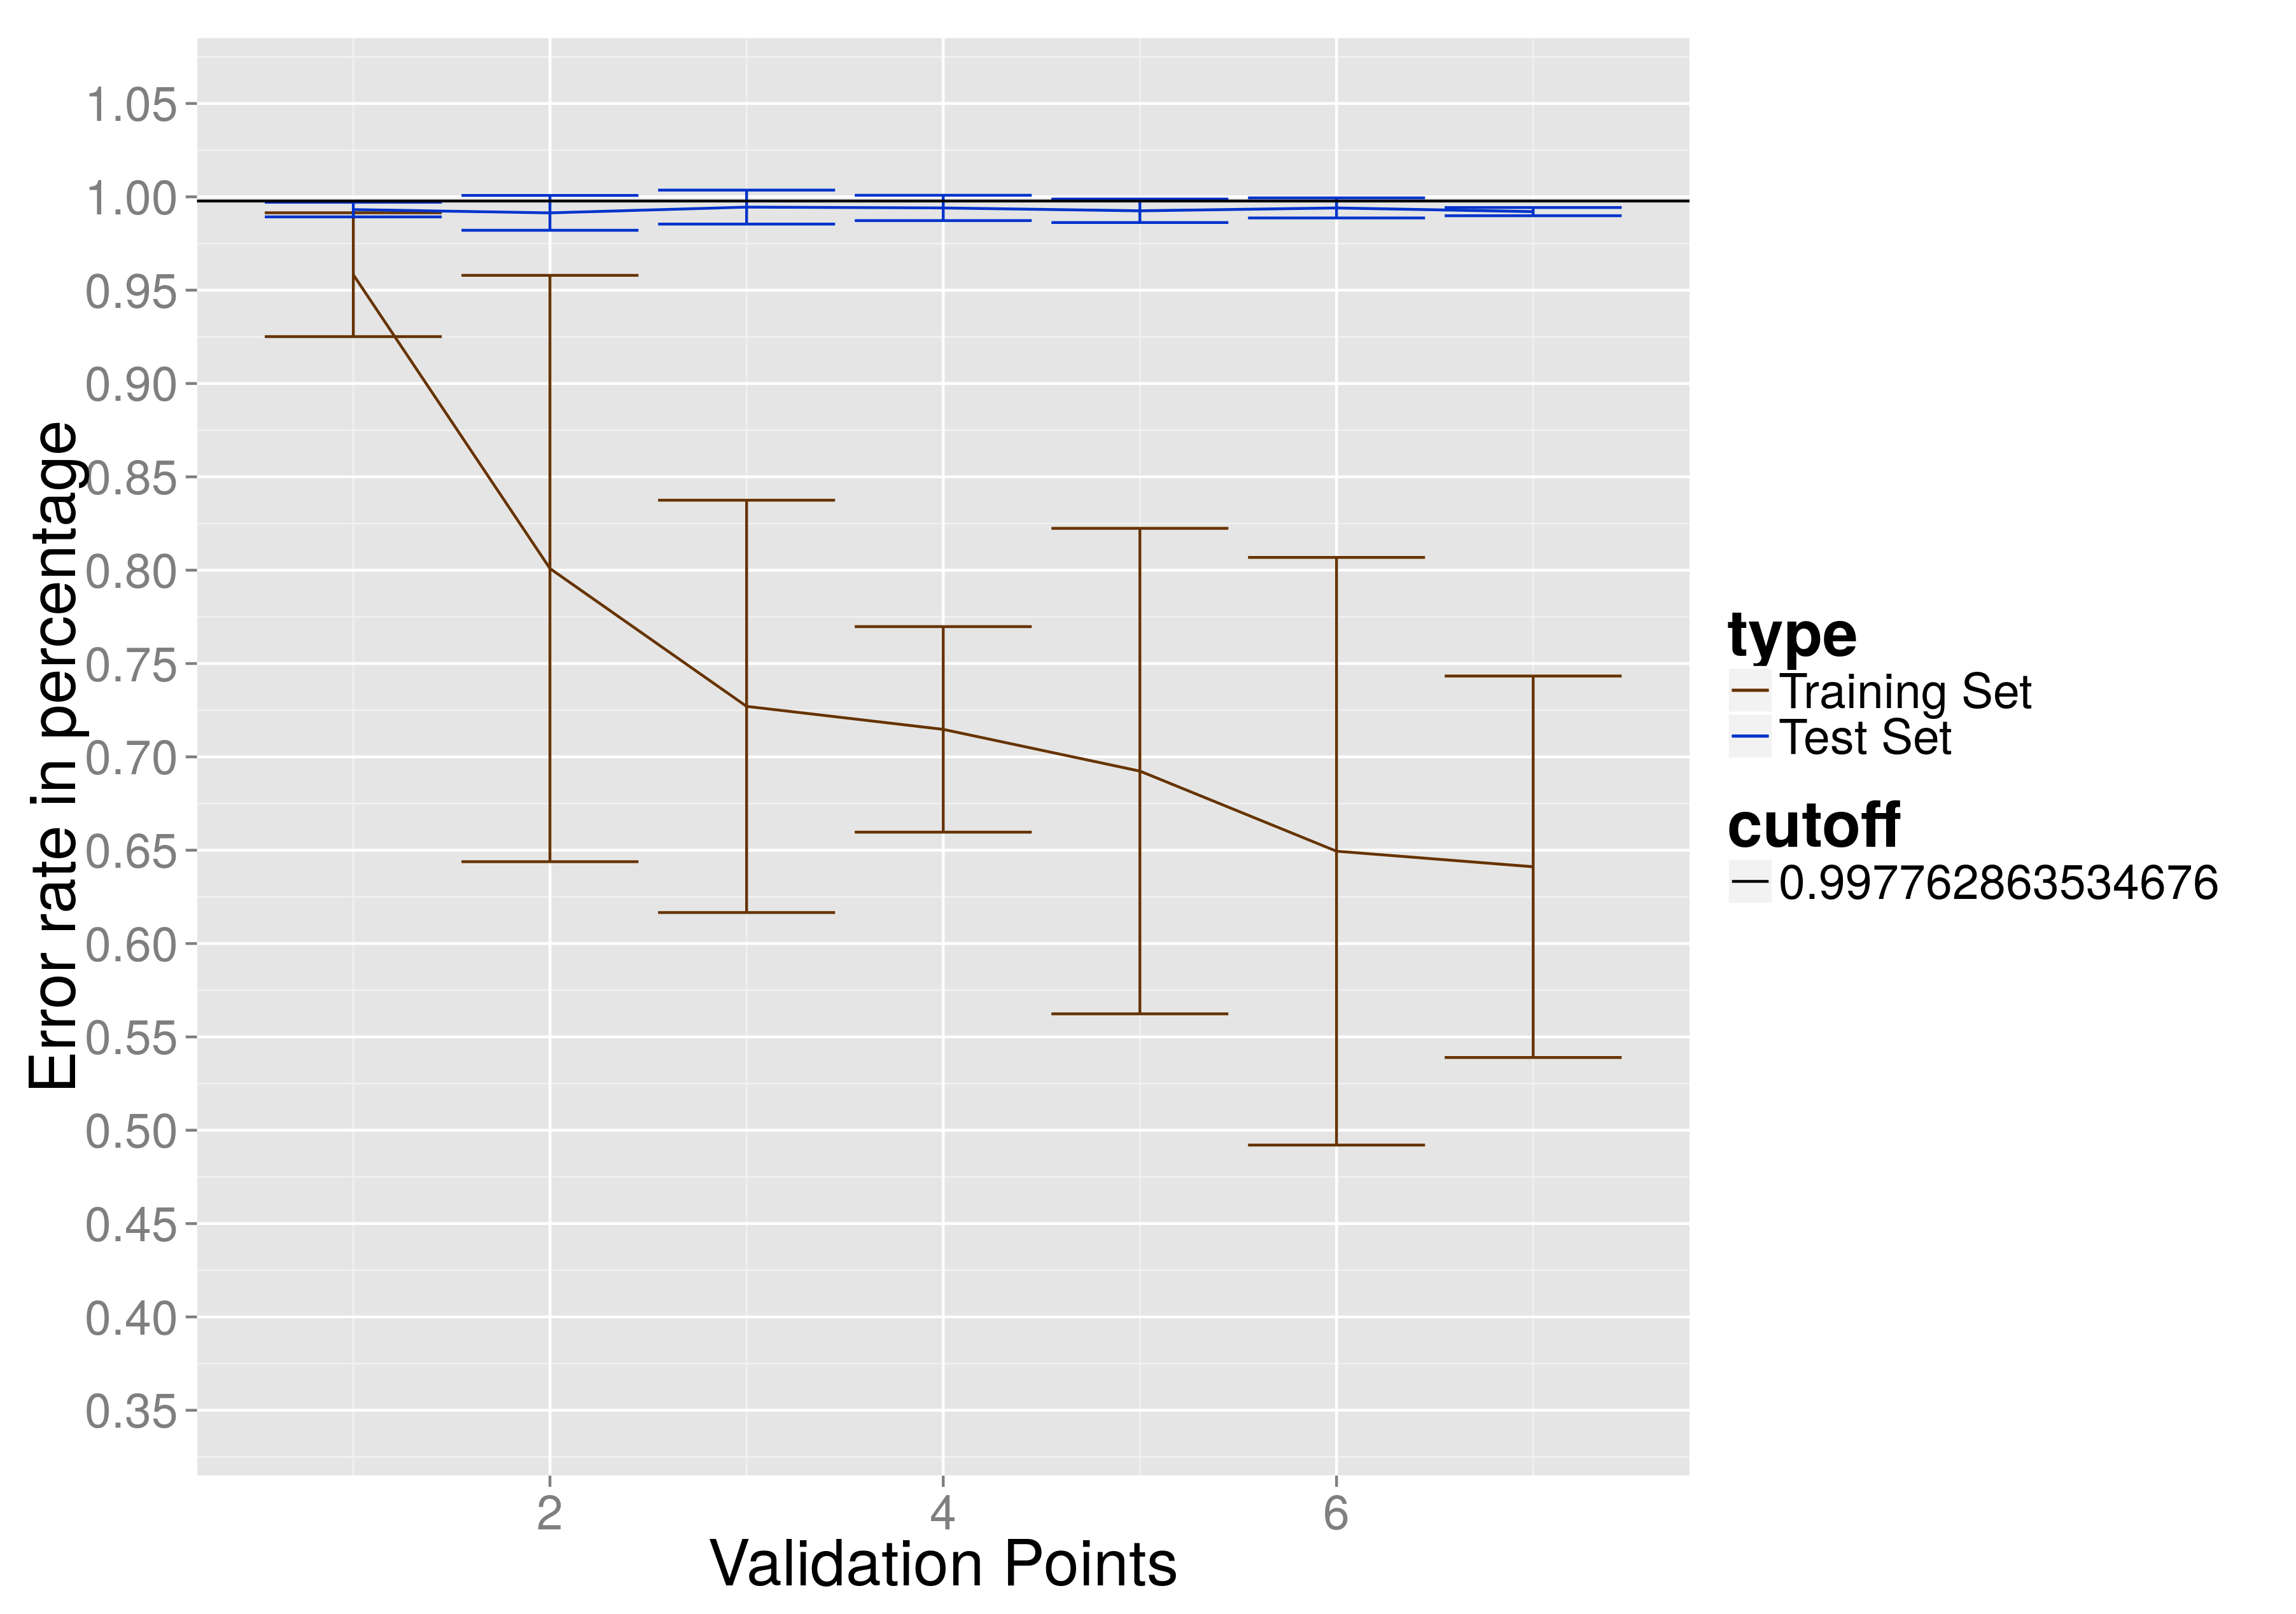
\includegraphics[width=0.95\linewidth]{Images/DNNraw}
      \caption{Without preprocessing}
      \label{fig:nn-resized}
    \end{subfigure}%
    \begin{subfigure}{.5\linewidth}
      \centering
      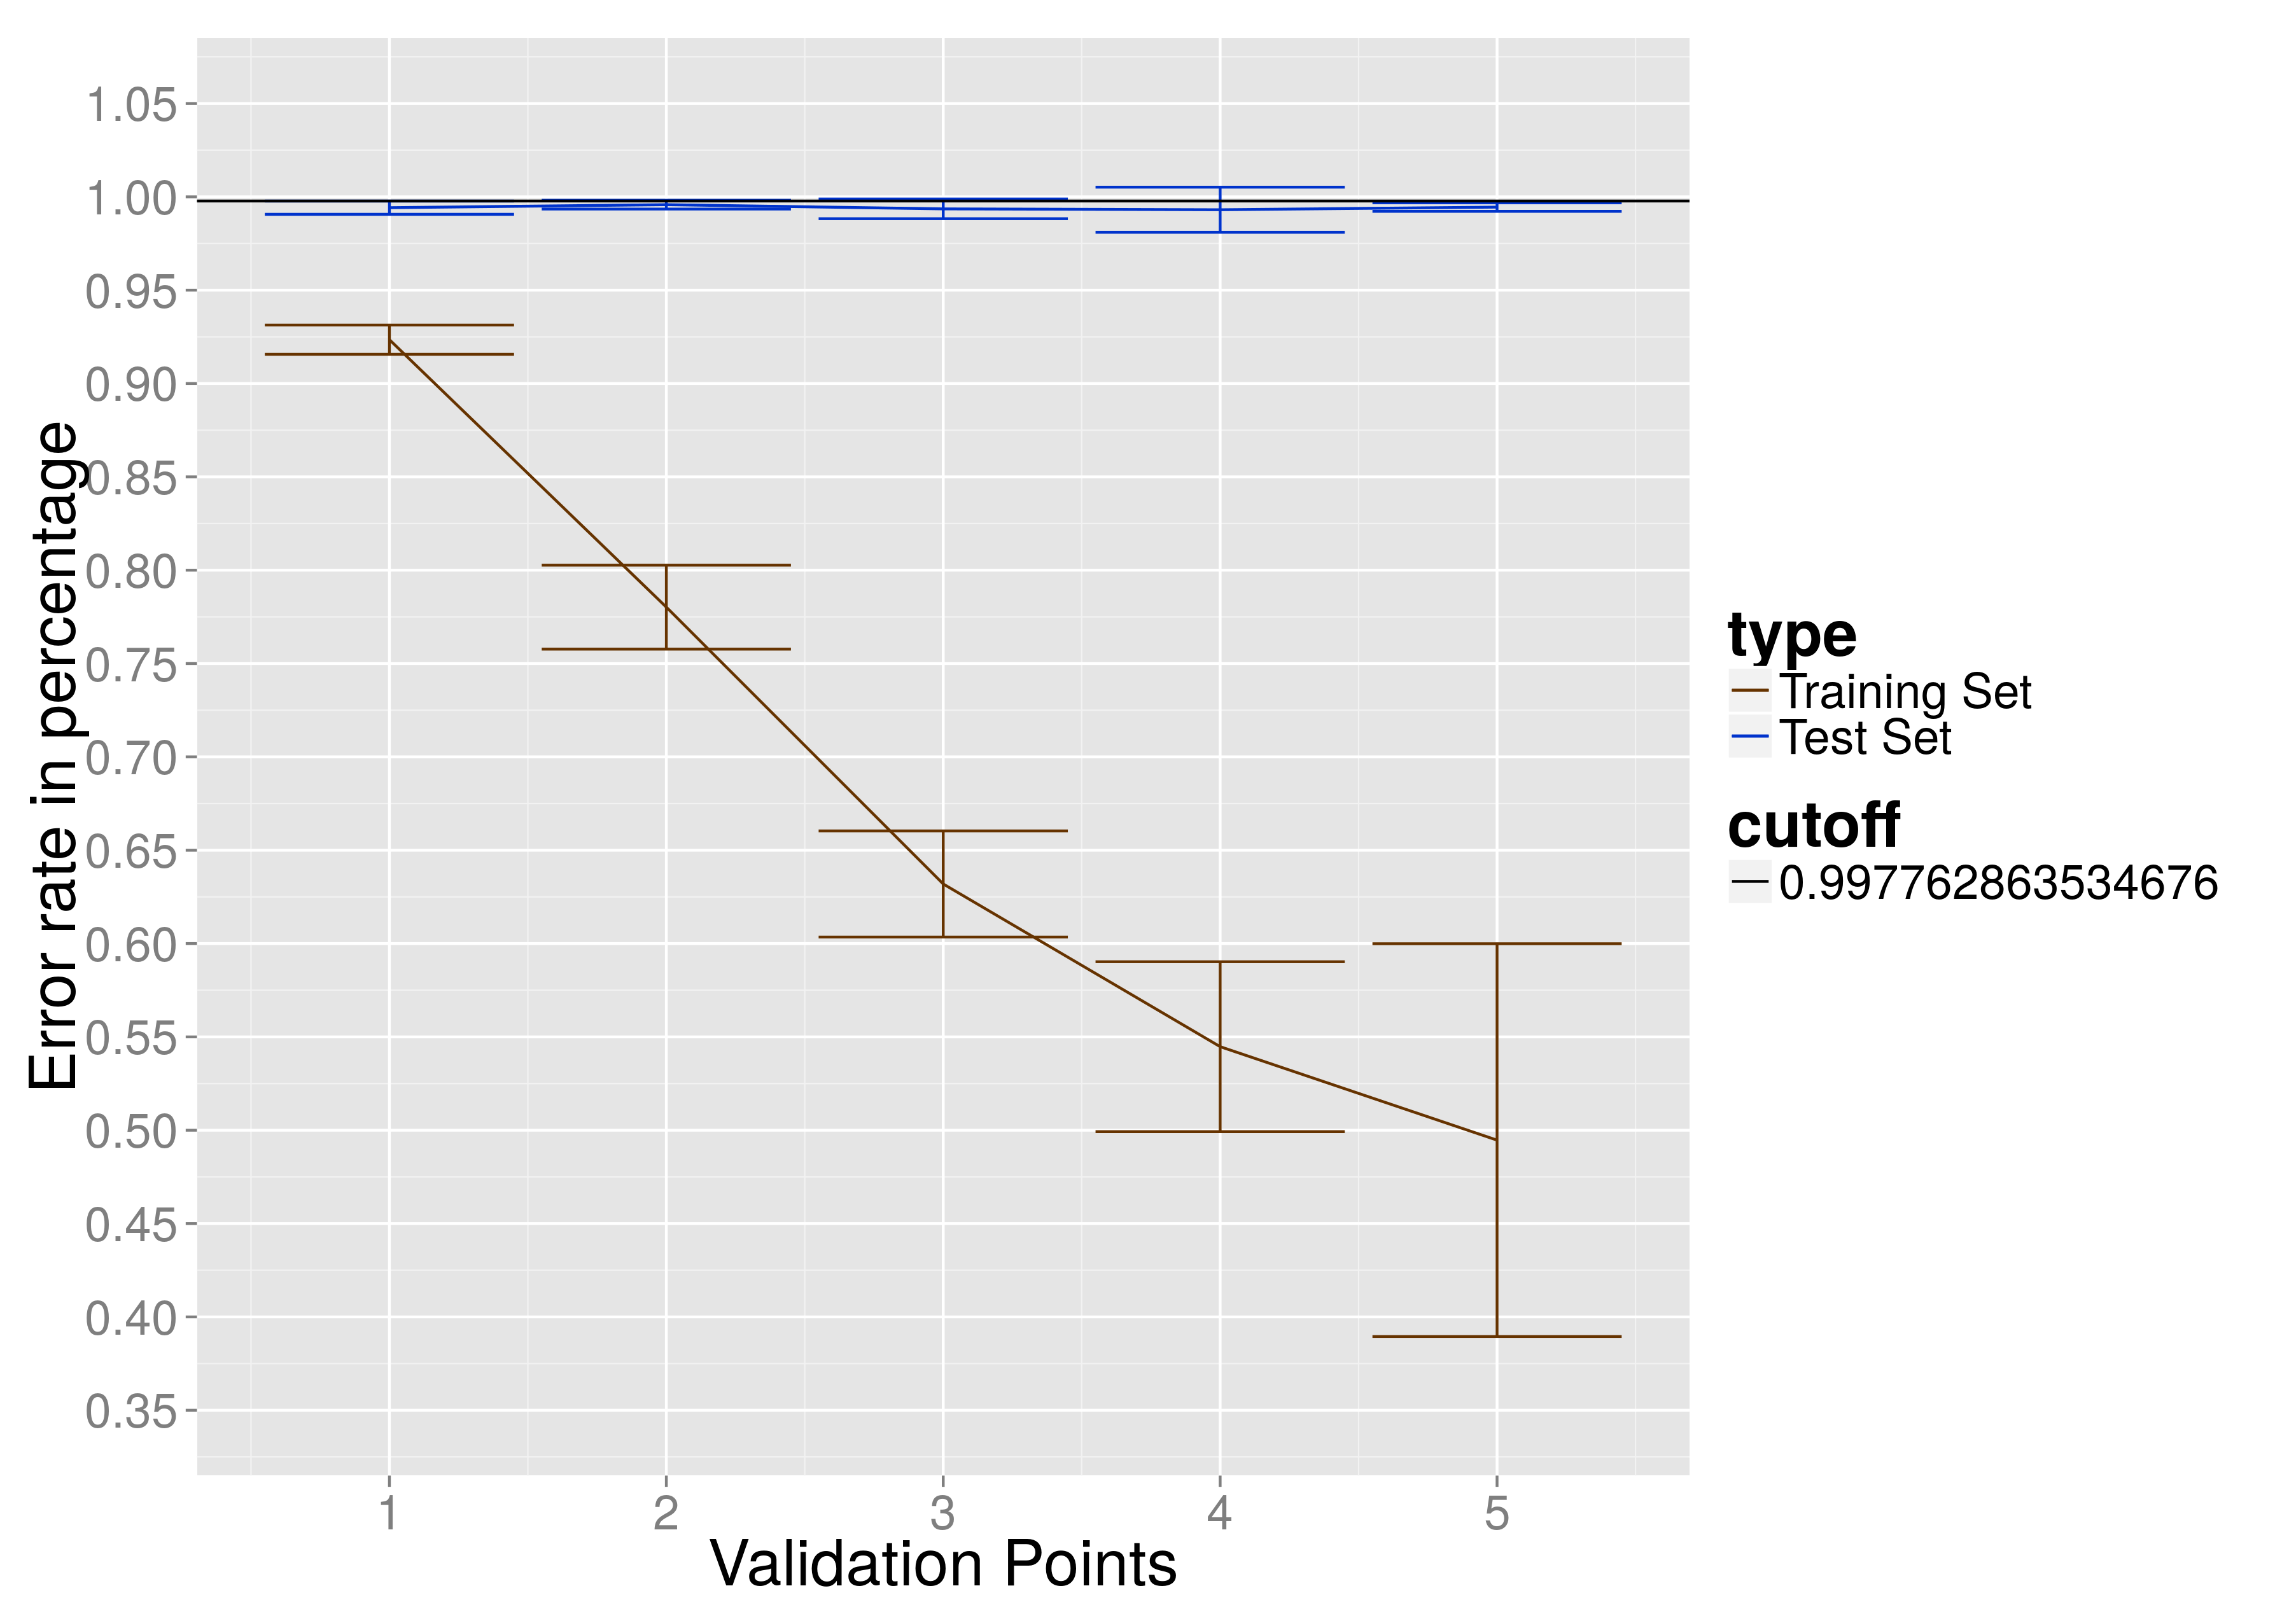
\includegraphics[width=0.95\linewidth]{Images/DNNpreprocessed}
      \caption{With preprocessing}
      \label{fig:nn-preprocessed}
    \end{subfigure}
  \caption{The results for Neural Network}
  \label{fig:neural-network}
\end{figure*}

\paragraph{The Preprocessed Data}
in Figure \ref{fig:nn-preprocessed} contains the same graph scheme as explained in previous paragraph in \ref{subsubsec:neuralnetwork}. 

The test set \emph{do not} have a significant better performance than random selection
, see Table \ref{tab:result-conclusion}.

The training set do have a \emph{significant better performance} against the model compared to the test set.

\subsubsection{Result Conclusion}
The results for the four different experiments shows that only Random Forest on the resized data stands out as an \emph{significant better performance} compared to random selection.

\begin{table}
  \caption{Probability for difference to random selecting for best performant validation point of each model and data input}
  \label{tab:result-conclusion}
  \begin{tabularx}{0.9\linewidth}{|X|X|l|} \hline
    \emph{Model}   & \emph{Data}               & \emph{Confidence} \\ \hline
    Random Forest  & Only Resized              & \(99.71 \%\)      \\ \hline
    Random Forest  & Preprocessed and Resized  & \(91.59 \%\)      \\ \hline
    Neural Network & Only Resized              & \(89.61 \%\)      \\ \hline
    Neural Network & Preprocessed and  Resized & \(78.50 \%\)      \\ \hline
  \end{tabularx}
\end{table}

\label{subsec:evaluation}
